\documentclass[aspectratio=169]{beamer}
\usepackage{pgf}
\usepackage{colortbl,tabularx,mathrsfs,calligra,xcolor}
\usepackage{amsmath,amsfonts,amssymb,amsthm}
\usepackage{ragged2e}
\usepackage{setspace}
\usepackage{filecontents}
\usepackage{caption}
\usepackage{subcaption}
\usepackage{contour}
\usepackage{fancybox}
\usepackage{wrapfig}
\usepackage{multirow}
\usepackage{multicol}
\usepackage{tikz, pgfplots, tkz-euclide,calc}
    \usetikzlibrary{patterns,snakes,shapes.arrows}
\usepackage{listings}
\usepackage{enumitem}
\usepackage{pifont}
\usepackage[scaled]{berasans}
    \renewcommand*\familydefault{\sfdefault}  %% Only if the base font of the document is to be sans serif
\usepackage[T1]{fontenc}
\usepackage{hyperref}
\hypersetup{
    filecolor=magenta,      
    urlcolor=cyan,
    pdftitle={Overleaf Example},
    pdfpagemode=FullScreen,
    }
\renewcommand*\familydefault{\sfdefault} %% Only if the base font of the document is to be sans serif

\graphicspath{{C:/Users/teoso/OneDrive/Documents/Asisten Dosen & Lab/Asisten Laboratorium/Alpro 1/PPT/Graphicx/}}

\definecolor{HIMAmuda}{HTML}{01D1FD}
\definecolor{HIMAtua}{HTML}{02016A}
\definecolor{HIMAabu}{HTML}{CBCBCC}
\definecolor{PastelGreen}{HTML}{77DD77}
\definecolor{pgray}{rgb}{0.5,0.5,0.5}
\definecolor{pblue}{rgb}{0.13,0.13,1}
\definecolor{pgreen}{rgb}{0,0.5,0}
\definecolor{pred}{rgb}{0.9,0,0}
\definecolor{pgrey}{rgb}{0.46,0.45,0.48}
\definecolor{pcyan}{HTML}{D4EFFC}
\definecolor{lblue}{HTML}{00AEEF}
\definecolor{input}{HTML}{AAE1FA}
\definecolor{bg}{rgb}{0.95, 0.95, 0.92}

\usepackage{listings}

\lstdefinestyle{standard}{
    language            =Java,
    showspaces          =false,
    showtabs            =false,
    breaklines          =true,
    showstringspaces    =false,
    breakatwhitespace   =true,
    commentstyle        =\color{pgray},
    keywordstyle        =\color{pblue},
    stringstyle         =\color{pgreen},
    basicstyle          =\small\ttfamily,
    frame               =single,
    backgroundcolor     =\color{bg},
    escapeinside        ={(*}{*)},
    numbers             = left, % {none, left, right}
    numberstyle         = \scriptsize\color{black},
    numbersep           = -8pt,
    }

\lstset{style=standard}

\usetheme{Madrid}

\setbeamercolor{palette primary}{bg=HIMAtua,fg=white}
\setbeamercolor{palette secondary}{bg=HIMAmuda,fg=black}
\setbeamercolor{palette tertiary}{bg=HIMAabu,fg=black}
\setbeamercolor{palette quaternary}{bg=HIMAmuda,fg=white}
\setbeamercolor{structure}{fg=HIMAmuda} % itemize, enumerate, etc
\setbeamercolor{section in toc}{fg=HIMAtua} % TOC sections
\setbeamercolor{block title alerted}{fg=white,bg=magenta}
\setbeamercolor{block body alerted}{fg=black!90,bg=pink}

\usefonttheme{professionalfonts}
\setbeamertemplate{theorems}[numbered]
\setbeamertemplate{itemize items}[circle]

\usebackgroundtemplate{%
\tikz[overlay,remember picture] \node[opacity=0.1, at=(current page.center)]{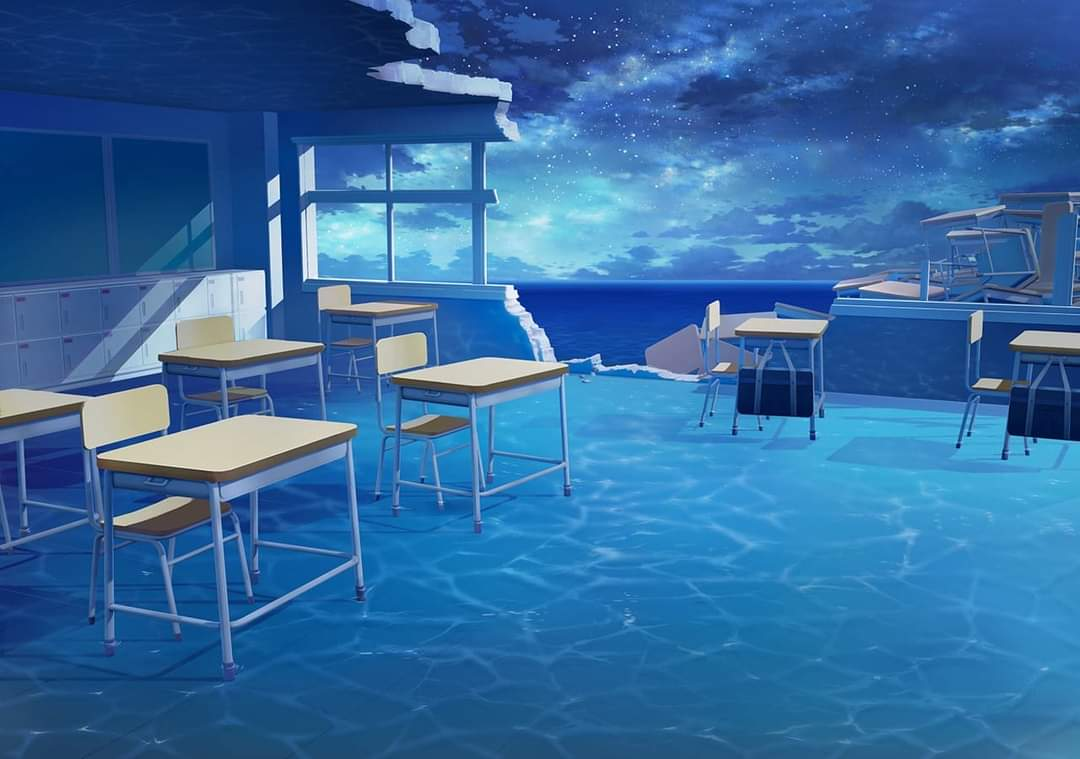
\includegraphics[width=\paperwidth]{plana class}};
}

\renewcommand\thesubfigure{\arabic{subfigure}}
\newtheorem*{funfact}{Fun Fact}
\newtheorem{latihan}{Latihan}
\newtheorem*{definisi}{Definisi}
\newtheorem{teorema}{Teorema}
\theoremstyle{definition}
\newtheorem*{contoh}{Contoh}
\newcommand{\R}{\mathbb{R}}

\AtBeginEnvironment{funfact}{%
  \setbeamercolor{block title}{fg=white,bg=PastelGreen} % Set title background to pastel green and text to white
  \setbeamercolor{block body}{parent=normal text,bg=PastelGreen!30!white} % Set body background to a lighter pastel green
}
\AtBeginEnvironment{definisi}{
    \setbeamercolor{block title}{fg=white,bg=HIMAtua}
    \setbeamercolor{block body}{parent=normal text,bg=HIMAtua!30!white}
}
\AtBeginEnvironment{teorema}{
    \setbeamercolor{block title}{bg=darkgray,fg=white}
    \setbeamercolor{block body}{parent=pallette tertiary,bg=HIMAabu!30!white}
}


\author[Tew \& Haf]{Hafidz Mulia\\Teosofi Hidayah Agung}
\date{9 September 2024}
\title[Alpro 1 - Week 1]{Pengenalan Bahasa Pemrograman Java}
\institute[Matematika ITS]{Departemen Matematika\\ Institut Teknologi Sepuluh Nopember}
\titlegraphic{{
\includegraphics[scale=0.02]{M.png}$\quad$
\includegraphics[scale=0.2]{Provicom.png}}}

\begin{document}
    {\usebackgroundtemplate{
        \tikz[overlay,remember picture] \node[opacity=0.2, at=(current page.center)]{
\includegraphics[width=\paperwidth]{Java bg}};}
    \begin{frame}
        \titlepage
    \end{frame}
    }

    {\usebackgroundtemplate{
     \tikz[overlay,remember picture] \node[opacity=0.1, at=(current page.center)]{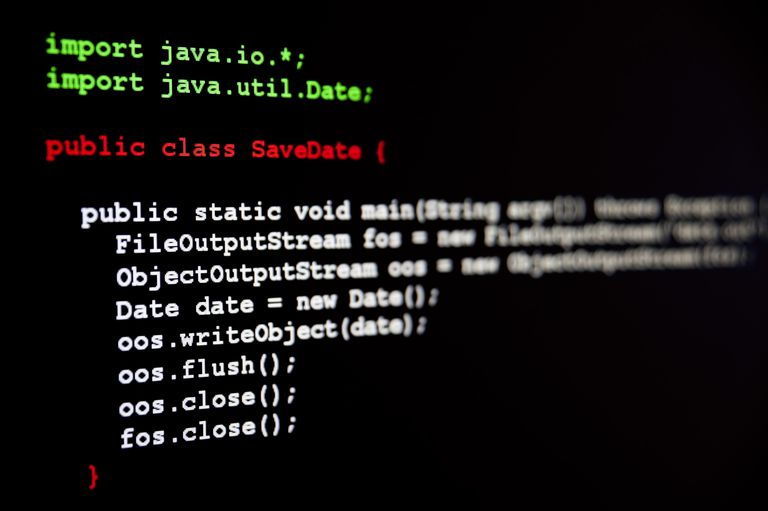
\includegraphics[width=\paperwidth]{Java code}};}
    \begin{frame}{Daftar isi}
        \tableofcontents
    \end{frame}
    }

    \section{Apa itu Java?}
    \begin{frame}
        \frametitle{\insertsection}
        \begin{block}{Backstory}
            Awalnya nama bahasa ini adalah "Oak" (yang main Minecraft pasti tau). Namun karena ada masalah hak cipta, maka nama brand ini perlu diganti. Singkat cerita, para developer berdiskusi di sebuah kafe dan saat itu mereka memesan kopi yang biji kopinya berasal dari pulau Jawa. Dari situlah mereka mendapat inspirasi untuk mengganti nama bahasa ini menjadi "Java".
        \end{block}
        \begin{figure}[h!]
            \centering
            
\includegraphics[width=0.1\textwidth]{Java logo}
            \caption{Logo Java}
        \end{figure}
    \end{frame}

    \begin{frame}
        \frametitle{\insertsection}
        \begin{definisi}
            Java adalah bahasa pemrograman yang diciptakan oleh James Gosling pada tahun 1991 saat masih bergabung di Sun Microsystems, yang saat ini merupakan bagian dari Oracle dan dirilis tahun 1995. Java adalah bahasa pemrograman yang bersifat \textit{high-level} dan \textit{object-oriented}. 
        \end{definisi}
        \begin{funfact}
            Bahasa pemrograman digunakan untuk menjalankan komputer, sebaliknya juga komputer digunakan untuk menjalankan bahasa pemrograman.\\~\\

            \onslide<2->{\textbf{Menurut kalian lebih dulu mana yang diciptakan? Bahasa pemrograman atau komputer?}}
        \end{funfact}
    \end{frame}

    \section{Kenapa harus Java?}
    \begin{frame}
        \frametitle{\insertsection}
        \begin{block}{Motivasi}
            \begin{itemize}[label=$\circ$]
                \item Apa saja kelebihan Java?
                \item Kenapa tidak Python? kan bahasa paling populer
                \item Whort it gak sih belajar Java?
            \end{itemize}
        \end{block}
    \end{frame}

    \begin{frame}
        \frametitle{\insertsection}
        \begin{figure}[h!]
            \centering
            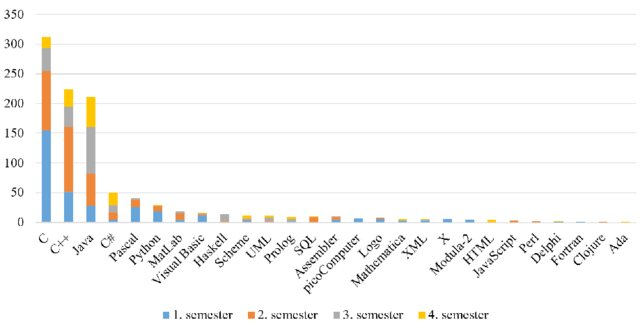
\includegraphics[width=0.7\textwidth]{Data Bahasa Pemrograman}
            \caption{\small Data Penggunaan Bahasa Pemrograman di Beberapa Kampus Eropa}
        \end{figure}
        SC: \href{https://www.researchgate.net/publication/309176375_Introductory_Programming_Subject_in_European_Higher_Education}{Introductory Programming Subject in European Higher Education}
    \end{frame}

    \begin{frame}[fragile]
        \frametitle{\insertsection}
        \begin{alertblock}{Kenapa bukan Python?}
            Bahasa seperti C atau Java memerlukan pemahaman yang lebih mendalam tentang konsep seperti manajemen memori dan tipe data. kurangnya aturan sintaksis yang ketat pada Python dapat menyebabkan kebiasaan pengkodean yang buruk jika tidak dipelajari dengan benar.
        \end{alertblock}
        \onslide<2->\begin{lstlisting}[caption={Masalah dalam deklarasi variabel}]
    // Eror di java namun tidak di Python
    x = 5;
    // Tidak eror di Java maupun Python
    int x = 5;
        \end{lstlisting}
    \end{frame}

    \section{Pengenalan Netbeans}
    \begin{frame}
        \frametitle{\insertsection}
        \begin{block}{IDE}
            Integrated Development Environment (IDE) adalah sebuah perangkat lunak yang digunakan untuk mengembangkan aplikasi perangkat lunak. IDE biasanya terdiri dari \textit{text editor}, \textit{compiler}, \textit{debugger}, dan \textit{build automation tools}.
        \end{block}
        \begin{block}{Netbeans}
            NetBeans adalah IDE yang digunakan untuk mengembangkan aplikasi Java. NetBeans memiliki fitur \textit{code completion}, \textit{syntax highlighting}, \textit{code refactoring}, dan \textit{version control}.
        \end{block}
    \end{frame}

    \begin{frame}
        \frametitle{\insertsection}
        \begin{exampleblock}{Project}
            Satuan besar yang mencakup seluruh kode sumber, file konfigurasi, dependensi, serta aset yang dibutuhkan untuk membangun aplikasi atau sistem.
        \end{exampleblock}
        \begin{exampleblock}{Package}
            Direktori yang berisi kelas-kelas Java yang terkait. Package digunakan untuk mengelompokkan kelas-kelas Java yang memiliki fungsi yang sama.
        \end{exampleblock}
        \begin{exampleblock}{Class}
            Struktur dasar dari Java yang digunakan untuk membuat objek. Class berisi properti dan \textit{method} yang digunakan untuk mendefinisikan objek.
        \end{exampleblock}
    \end{frame}

    \setbeamercolor{block title}{bg=brown,fg=white} % Block title background brown, text white
    \setbeamercolor{block body}{bg=brown!30,fg=black}  
    \section{Ngoding TIME!}
    \begin{frame}[fragile]
        \frametitle{\insertsection}
        \begin{block}{Hello, World!}
            Program pertama yang biasanya dibuat oleh programmer ketika belajar bahasa pemrograman baru adalah program "Hello, World!".
        \end{block}
        \begin{lstlisting}
    public class Main {
        public static void main(String[] args) {
            System.out.println("Hello, World!");
        }
    }
        \end{lstlisting}
    \end{frame}

    \begin{frame}
        \frametitle{\insertsection}
        \begin{block}{Silahkan Coba}
            Buatlah program yang menampilkan nama, NRP, Asal, dan Funfact
        \end{block}
    \end{frame}
\end{document}